\documentclass[tikz,border=8pt]{standalone}
% Shared look for every TikZ diagram. Load with % Shared look for every TikZ diagram. Load with % Shared look for every TikZ diagram. Load with \input{../../tools/tikz-style.tex}
\usepackage[T1]{fontenc}
\usepackage{lmodern}
\renewcommand{\sfdefault}{lmr}  % diagrams use the same serif as the text
\usetikzlibrary{arrows.meta, positioning, shapes.geometric, calc, fit, backgrounds}
\definecolor{cblue}{HTML}{4C78A8}
\definecolor{corange}{HTML}{F58518}
\definecolor{cgreen}{HTML}{54A24B}
\definecolor{cred}{HTML}{E45756}
\definecolor{cpurple}{HTML}{B279A2}
\definecolor{cgrey}{HTML}{6B6B6B}
\tikzset{
  every picture/.style={font=\sffamily, line width=1.2pt},
  box/.style={draw=#1, fill=#1!12, rounded corners=4pt, align=center, inner sep=7pt, minimum height=1.1cm},
  box/.default=cgrey,
  arrow/.style={-{Stealth[length=3mm]}, draw=cgrey, line width=1.4pt},
  title/.style={font=\sffamily\bfseries\Large},
  note/.style={font=\sffamily\small, text=cgrey, align=center},
}
\AtBeginDocument{\hyphenpenalty=10000 \exhyphenpenalty=10000}

\usepackage[T1]{fontenc}
\usepackage{lmodern}
\renewcommand{\sfdefault}{lmr}  % diagrams use the same serif as the text
\usetikzlibrary{arrows.meta, positioning, shapes.geometric, calc, fit, backgrounds}
\definecolor{cblue}{HTML}{4C78A8}
\definecolor{corange}{HTML}{F58518}
\definecolor{cgreen}{HTML}{54A24B}
\definecolor{cred}{HTML}{E45756}
\definecolor{cpurple}{HTML}{B279A2}
\definecolor{cgrey}{HTML}{6B6B6B}
\tikzset{
  every picture/.style={font=\sffamily, line width=1.2pt},
  box/.style={draw=#1, fill=#1!12, rounded corners=4pt, align=center, inner sep=7pt, minimum height=1.1cm},
  box/.default=cgrey,
  arrow/.style={-{Stealth[length=3mm]}, draw=cgrey, line width=1.4pt},
  title/.style={font=\sffamily\bfseries\Large},
  note/.style={font=\sffamily\small, text=cgrey, align=center},
}
\AtBeginDocument{\hyphenpenalty=10000 \exhyphenpenalty=10000}

\usepackage[T1]{fontenc}
\usepackage{lmodern}
\renewcommand{\sfdefault}{lmr}  % diagrams use the same serif as the text
\usetikzlibrary{arrows.meta, positioning, shapes.geometric, calc, fit, backgrounds}
\definecolor{cblue}{HTML}{4C78A8}
\definecolor{corange}{HTML}{F58518}
\definecolor{cgreen}{HTML}{54A24B}
\definecolor{cred}{HTML}{E45756}
\definecolor{cpurple}{HTML}{B279A2}
\definecolor{cgrey}{HTML}{6B6B6B}
\tikzset{
  every picture/.style={font=\sffamily, line width=1.2pt},
  box/.style={draw=#1, fill=#1!12, rounded corners=4pt, align=center, inner sep=7pt, minimum height=1.1cm},
  box/.default=cgrey,
  arrow/.style={-{Stealth[length=3mm]}, draw=cgrey, line width=1.4pt},
  title/.style={font=\sffamily\bfseries\Large},
  note/.style={font=\sffamily\small, text=cgrey, align=center},
}
\AtBeginDocument{\hyphenpenalty=10000 \exhyphenpenalty=10000}

\begin{document}
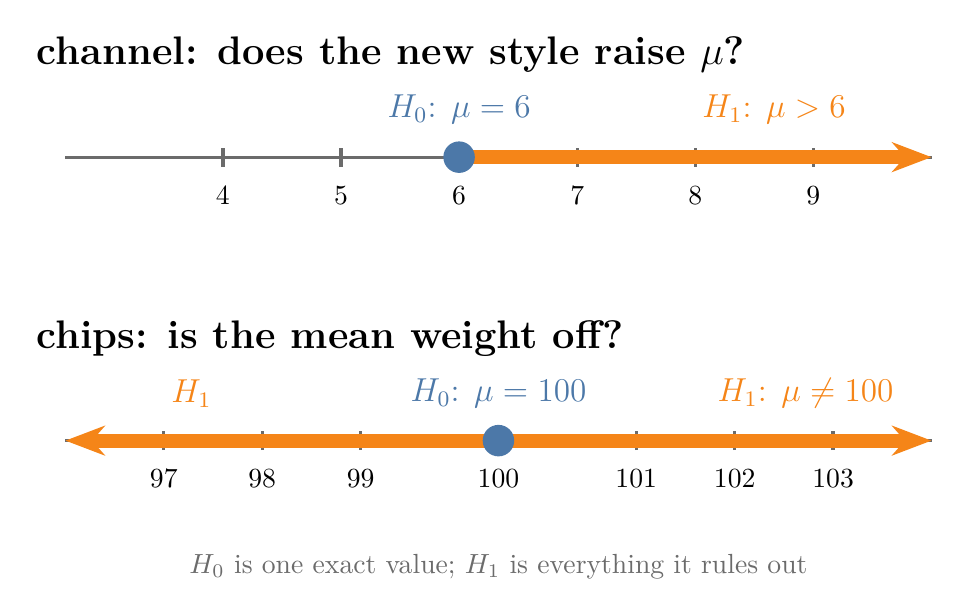
\begin{tikzpicture}[every node/.append style={font=\sffamily\large}]
  % channel: right-tailed
  \node[title, anchor=west] at (-0.5,1.3) {channel: does the new style raise $\mu$?};
  \draw[cgrey, line width=1pt] (0,0) -- (11,0);
  \foreach \v/\x in {4/2, 5/3.5, 6/5, 7/6.5, 8/8, 9/9.5} {\draw[cgrey] (\x,-0.12) -- (\x,0.12); \node[below=4pt, font=\sffamily] at (\x,-0.1) {\v};}
  \draw[corange, line width=5pt, -{Stealth[length=5mm]}] (5.15,0) -- (11,0);
  \fill[cblue] (5,0) circle (0.2);
  \node[text=cblue, above=8pt] at (5,0) {$H_0$: $\mu = 6$};
  \node[text=corange, above=8pt] at (9,0) {$H_1$: $\mu > 6$};
  % chips: two-tailed
  \begin{scope}[yshift=-3.6cm]
  \node[title, anchor=west] at (-0.5,1.3) {chips: is the mean weight off?};
  \draw[cgrey, line width=1pt] (0,0) -- (11,0);
  \foreach \v/\x in {97/1.25, 98/2.5, 99/3.75, 100/5.5, 101/7.25, 102/8.5, 103/9.75} {\draw[cgrey] (\x,-0.12) -- (\x,0.12); \node[below=4pt, font=\sffamily] at (\x,-0.1) {\v};}
  \draw[corange, line width=5pt, -{Stealth[length=5mm]}] (5.35,0) -- (0,0);
  \draw[corange, line width=5pt, -{Stealth[length=5mm]}] (5.65,0) -- (11,0);
  \fill[cblue] (5.5,0) circle (0.2);
  \node[text=cblue, above=8pt] at (5.5,0) {$H_0$: $\mu = 100$};
  \node[text=corange, above=8pt] at (1.6,0) {$H_1$};
  \node[text=corange, above=8pt] at (9.4,0) {$H_1$: $\mu \neq 100$};
  \end{scope}
  \node[note, font=\sffamily] at (5.5,-5.2) {$H_0$ is one exact value; $H_1$ is everything it rules out};
\end{tikzpicture}
\end{document}
